% \usepackage{hyperref}

% %%%% For camera-ready, use this
% %\documentclass[sigconf]{aamas}

% \usepackage{listings}
% % \usepackage{xcolor}

% \definecolor{codegreen}{rgb}{0,0.6,0}
% \definecolor{codegray}{rgb}{0.5,0.5,0.5}
% \definecolor{codepurple}{rgb}{0.58,0,0.82}
% \definecolor{backcolour}{rgb}{0.95,0.95,0.92}

% \lstdefinestyle{mystyle}{
%     backgroundcolor=\color{backcolour},   
%     commentstyle=\color{codegreen},
%     keywordstyle=\color{magenta},
%     numberstyle=\tiny\color{codegray},
%     stringstyle=\color{codepurple},
%     basicstyle=\footnotesize,
%     breakatwhitespace=false,         
%     breaklines=true,                 
%     captionpos=b,                    
%     keepspaces=true,                 
%     numbers=left,                    
%     numbersep=5pt,                  
%     showspaces=false,                
%     showstringspaces=false,
%     showtabs=false,                  
%     tabsize=2
% }

% \lstset{style=mystyle}

% % --- Tickz
% \usepackage{physics}
% \usepackage{tikz}
% \usepackage{amsmath}
% \usepackage{mathdots}
% % \usepackage{yhmath}
% \usepackage{cancel}
% \usepackage{color}
% \usepackage{siunitx}
% \usepackage{array}
% \usepackage{multirow}
% % \usepackage{amssymb}
% \usepackage{gensymb}
% \usepackage{tabularx}
% \usepackage{extarrows}
% \usepackage{booktabs}
% \usetikzlibrary{fadings}
% \usetikzlibrary{patterns}
% \usetikzlibrary{shadows.blur}
% \usetikzlibrary{shapes}

% % ---------

% \usepackage{balance} % for balancing columns on the final page
% \usepackage{csquotes}
% % \usepackage{cite}
% \newcommand{\probP}{\text{I\kern-0.15em P}}
% \usepackage{etoolbox}
% \patchcmd{\thebibliography}{\section*{\refname}}{}{}{}
% % \usepackage{amsthm,amssymb,amsfonts}

% \usepackage[T1]{fontenc}
% \usepackage{graphicx}
% \usepackage{color}
% % \renewcommand\UrlFont{\color{blue}\rmfamily}

% \usepackage[inline, shortlabels]{enumitem}
% \usepackage{tabularx}
% \usepackage{caption}
% \usepackage{listings}
% \usepackage{stfloats}
% \usepackage{titlesec}
% \usepackage{ragged2e}
% % \usepackage[hyphens]{url}
% \usepackage[linesnumbered,ruled,vlined]{algorithm2e}
% \usepackage{float}
% \usepackage[english]{babel}
% \addto\extrasenglish{  
%     \def\figureautorefname{Figure}
%     \def\tableautorefname{Table}
%     \def\algorithmautorefname{Algorithm}
%     \def\sectionautorefname{Section}
%     \def\subsectionautorefname{Subsection}
%     \def\proofoutlineautorefname{Proof Outline}
% }



\section{Introduction}

% Contexte
L'apprentissage par renforcement multi-agents (MARL) permet de découvrir une politique commune qui contrôle les comportements des agents afin qu'ils puissent atteindre un objectif global dans un environnement spécifique.
Cette politique commune dicte non seulement les actions individuelles des agents, mais gère également leurs interactions entre eux, et potentiellement avec tous les autres agents, sans aucune notion préconçue d'une organisation prédéfinie.

Dans les environnements qui nécessitent une interaction sociale entre les agents pour atteindre de manière optimale l'objectif global, les agents peuvent converger de telle sorte qu'ils présentent des ensembles récurrents de comportements similaires au cours de différents épisodes de test.
Ces ensembles distincts de comportements peuvent présenter des propriétés de spécialisation, de complémentarité et de stabilité, ce qui les rend similaires à des rôles implicites. De plus, les trajectoires des agents assumant ces rôles « implicites » peuvent présenter des similitudes, telles que des observations récurrentes à la fin de chaque épisode. Ces modèles récurrents dans l'historique des agents peuvent être interprétés comme des objectifs « implicites », suggérant que les agents peuvent chercher à les atteindre comme objectifs intermédiaires avant d'atteindre l'objectif global. Ces rôles implicites et ces objectifs implicites constituent le fondement d'une organisation structurelle et fonctionnelle « implicite » telle que définie dans $\mathcal{M}OISE^+$~\cite{Hubner2007}.

Cependant, il serait trompeur de supposer que tous les agents formés dans n'importe quel environnement peuvent être fidèlement comparés à une organisation structurelle et fonctionnelle. En effet, nous pouvons interpréter les comportements des agents formés en fonction de leur similitude avec la vision potentielle d'une organisation structurelle et fonctionnelle implicite, que nous définissons comme l'« adéquation organisationnelle ».
Si l'évaluation de l'adéquation organisationnelle serait utile pour déterminer dans quelle mesure les agents entraînés peuvent être naturellement expliqués en termes de rôles et d'objectifs, on pourrait également envisager l'approche inverse. En guidant ou en encourageant les agents à converger vers des organisations structurelles et fonctionnelles présentant une meilleure adéquation organisationnelle, nous visons à améliorer l'explicabilité et le contrôle dans le MARL.

\

% Problème
Partant de ces hypothèses, cet article vise à explorer plus en détail deux aspects clés :
\begin{enumerate*}[label={\roman*) },itemjoin={; \quad}]
    \item L'\textbf{évaluation de l'adéquation organisationnelle}, qui cherche à mesurer dans quelle mesure une politique commune s'aligne sur une organisation structurelle et fonctionnelle. Un défi important consiste ici à comprendre dans quelles conditions les agents peuvent être considérés comme formant une organisation structurelle et fonctionnelle, compte tenu des contraintes imposées par l'environnement, les objectifs et d'autres facteurs facultatifs.
    La littérature existante aborde souvent l'évaluation des politiques en termes de rôles ou d'objectifs~\cite{Isakov2024, Wen2024, Xie2024}, mais ces travaux manquent généralement d'une approche systématique et globale. Les méthodes actuelles offrent peu d'outils clairs pour mesurer quantitativement et qualitativement cette adéquation organisationnelle.
    \item Le \textbf{contrôle de l'adéquation organisationnelle}, qui vise à guider les agents vers des politiques conformes à une organisation structurelle et fonctionnelle grâce à des contraintes ou des incitations définies par l'utilisateur qui mettent en œuvre des rôles et des objectifs.
    Les principaux défis consistent à réduire l'espace de recherche des politiques, à améliorer la convergence et à garantir le respect des contraintes de sécurité.
    Les approches existantes dans ce domaine sont souvent insuffisantes pour permettre aux utilisateurs de définir et de gérer facilement l'application des spécifications organisationnelles de manière pratique dans un cadre MARL standard, sans s'appuyer sur des paradigmes tels que l'apprentissage par renforcement hiérarchique (HRL).
\end{enumerate*}

\

% Contribution
\noindent Nous présentons le cadre \textbf{MOISE+MARL}, qui intègre le cadre MARL du processus de décision markovien partiellement observable décentralisé (Dec-POMDP) avec le modèle organisationnel $\mathcal{M}OISE^+$~\cite{Hubner2007} grâce à des relations proposées. Ce cadre permet aux utilisateurs de définir manuellement la logique d'un rôle ou d'un objectif en s'appuyant sur des modèles basés sur des trajectoires pour décrire le comportement attendu d'un agent qui a adopté un objectif ou une mission. Une fois configurés, ils permettent aux utilisateurs d'appliquer un rôle à un agent, en ajoutant des contraintes qui influencent automatiquement les politiques des agents en mettant à jour dynamiquement l'espace d'action et en remodelant la fonction de récompense. Ce cadre comprend également une méthode appelée « évaluation basée sur la trajectoire dans MOISE+MARL » (TEMM), qui utilise des techniques d'apprentissage non supervisé pour généraliser les rôles implicites et les missions implicites à partir de trajectoires observées au cours de plusieurs épisodes de test. En mesurant l'écart entre les spécifications organisationnelles implicites déduites et les comportements réels, cette méthode permet une évaluation quantitative de l'adéquation organisationnelle. Il convient de noter que contrairement à l'apprentissage par renforcement hiérarchique, qui décompose les tâches en sous-tâches~\cite{Qi2024, Matsuyama2025, SaoMai2024}, notre approche s'appuie sur des rôles et des missions organisationnels explicites pour guider la coordination des agents de manière externe.

\

% Évaluation et conclusions
Nous avons évalué le cadre MOISE+MARL dans les scénarios suivants :
\begin{enumerate*}[label={\roman*) },itemjoin={; \quad}]
    \item Quatre environnements distincts, chacun devant aboutir à la formation de politiques conjointes avec différentes organisations implicites, afin d'évaluer la généralisation de l'applicabilité de MOISE+ MARL
    \item Quatre algorithmes MARL issus de plusieurs familles afin d'évaluer leur adéquation avec MOISE+ MARL pendant la formation et l'analyse postérieure
    \item Quatre ensembles de spécifications organisationnelles, un pour chaque environnement, afin de contraindre les agents de manière à imposer la conformité prévue pour l'évaluation manuelle et quantitative.
    \item Quatre ensembles de spécifications organisationnelles, un pour chaque environnement, afin de contraindre les agents de manière à garantir la conformité visée pour l'évaluation manuelle et quantitative.
\end{enumerate*}


Dans tous les environnements, nous avons observé que les agents ayant adopté des rôles se comportent comme prévu en fonction de leurs rôles, de manière corrélée avec une mesure quantitative de l'adéquation organisationnelle par TEMM. Les rôles et les missions déduits par TEMM correspondent étroitement aux spécifications prédéfinies, ce qui démontre la cohérence interne de MOISE+MARL, car les modifications de politique introduites par les spécifications organisationnelles sont efficacement capturées par TEMM.
Les résultats indiquent également que les algorithmes basés sur des politiques et sur la critique des acteurs sont particulièrement bien adaptés pour guider les agents vers des politiques stables. Cette stabilité permet aux agents de maintenir des comportements cohérents et cohérents d'un épisode à l'autre, ce qui est essentiel pour la génération d'une organisation implicite stable par TEMM. En revanche, les algorithmes basés sur la valeur ont montré une plus grande variabilité dans les comportements des agents.

\

% Structure de l'article
\noindent Le reste de l'article est organisé comme suit : \autoref{sec:related_works} présente des travaux relatifs à l'évaluation et au contrôle de l'adéquation organisationnelle. \autoref{sec:moise_marl_framework} présente le cadre MOISE+MARL. \autoref{sec:TEMM_algorithm} décrit la méthode TEMM. \autoref{sec:experimental_setup} décrit le protocole expérimental, en particulier les environnements et les algorithmes MARL. \autoref{sec:results} présente les résultats expérimentaux. Enfin, \autoref{sec:discussion_conclusion_future_work} discute et conclut sur l'évaluation et le contrôle de l'adéquation organisationnelle.


\section{Travaux connexes}
\label{sec:travaux_connexes}

Cette section explore les travaux liés à l'adéquation organisationnelle, tels que définis par les deux questions fondamentales présentées.

\subsection{Évaluation de l'adéquation organisationnelle}

Certains travaux peuvent être liés à l'inférence de rôles ou d'objectifs concernant la nécessité de calculer l'adéquation organisationnelle ou des concepts proches.
%
Wilson et al.~\cite{wilson2008learning} développent une méthode de transfert de rôles dans les MDP multi-agents, qui aide les agents à s'adapter en transférant des rôles entre différents environnements. Cependant, leur modèle manque d'abstraction des rôles, car il se concentre sur des rôles spécifiques liés à des tâches.
%
Berenji et Vengerov~\cite{berenji2000learning} étudient la coordination et l'inférence des rôles dans les missions de drones, améliorant la coopération grâce à la modélisation des dépendances entre agents. Bien qu'utile pour la coopération, leur approche reste spécifique à une tâche et ne fournit pas le calcul implicite des rôles nécessaire à l'adéquation organisationnelle.
%
Yusuf et Baber~\cite{yusuf2020inferential} utilisent le raisonnement inférentiel et les méthodes bayésiennes pour faciliter la coordination des tâches entre divers agents. Bien qu'efficace dans la coordination dynamique, leur cadre manque d'abstraction des rôles et ne mesure pas non plus l'alignement avec une structure organisationnelle plus large.
%
Serrino et al.~\cite{serrino2019finding} examinent l'inférence dynamique des rôles dans des contextes sociaux, où les agents déduisent les rôles à travers leurs interactions. Bien qu'ils permettent une compréhension flexible des rôles, leur approche se concentre sur les rôles opérationnels immédiats plutôt que sur les rôles implicites qui s'alignent sur les modèles organisationnels.

Si certains travaux explorent les concepts organisationnels dans le MARL, aucun ne traite explicitement du calcul de l'alignement organisationnel tel que nous le définissons. Notre concept d'adéquation organisationnelle nécessite un cadre qui évalue l'alignement avec des objectifs implicites.


\subsection{Contrôle de l'adéquation organisationnelle}
Le contrôle de l'adéquation organisationnelle implique d'aligner les politiques des agents sur une organisation prédéfinie, souvent à l'aide de contraintes ou d'incitations.
%
Achiam et al.~\cite{achiam2017cpo} introduisent le CPO, qui ajuste les politiques en tenant compte des contraintes de sécurité tout en maximisant les récompenses. MOISE+MARL, cependant, introduit des contraintes allant au-delà de la sécurité afin de façonner le comportement en fonction des attentes organisationnelles en guidant de manière externe l'apprentissage des agents.
%
Ray et al.~\cite{ray2019benchmarking} utilisent des multiplicateurs de Lagrange pour intégrer les contraintes dans la fonction de récompense, équilibrant ainsi la récompense et le respect des contraintes. MOISE+MARL étend cette approche en modifiant dynamiquement l'espace d'action afin de faire respecter les contraintes à différents niveaux, offrant ainsi un contrôle flexible sur les comportements des agents.
%
Une exploration sûre garantit que les agents apprennent tout en respectant les contraintes de sécurité. Garcia et al.~\cite{garcia2015comprehensive} présentent des méthodes pour maintenir une exploration sûre, et Alshiekh et al.~\cite{alshiekh2018safe} proposent un bouclier pour bloquer les actions dangereuses. MOISE+MARL va plus loin en utilisant des contraintes pour guider les agents vers des comportements qui correspondent aux rôles organisationnels.
%
Le HRL divise les tâches en sous-tâches, en fonction des hiérarchies organisationnelles. Ghavamzadeh et al.~\cite{ghavamzadeh2006hrl} illustrent que le HRL peut améliorer la coordination. MOISE+MARL impose des contraintes externes au MARL, offrant une granularité modulaire et générant des comportements affinés dans le respect des contraintes organisationnelles.
%
Le contrôle de la communication et de la coordination est essentiel pour garantir l'adéquation organisationnelle, en particulier dans les systèmes à grande échelle. Foerster et al.~\cite{foerster2018communication} proposent une coordination décentralisée grâce au partage des connaissances, permettant aux agents de fonctionner sans contrôle centralisé.

Contrairement au HRL, le cadre MOISE+MARL se distingue par l'intégration de contraintes organisationnelles externes qui influencent les agents dans un cadre MARL standard, permettant ainsi une granularité modulaire. Contrairement au Shielding ou au CPO, qui se concentrent généralement sur les contraintes de sécurité, MOISE+MARL va plus loin en s'appuyant sur des actions et des modifications de récompenses pour s'aligner sur les rôles. % MOISE+MARL vise à gérer l'évolutivité et l'adaptabilité en simplifiant les interactions des utilisateurs pour définir et appliquer un nombre réduit de spécifications organisationnelles.


\section{Le cadre MOISE+MARL}
\label{sec:moise_marl_framework}

Cette section présente le formalisme utilisé pour décrire le fonctionnement du cadre MOISE+MARL.

\subsection{Cadre de Markov pour MARL}

Pour appliquer les techniques MARL, nous nous appuyons sur le \textit{processus de décision markovien décentralisé partiellement observable} (Dec-POMDP) \cite{Oliehoek2016}. Les Dec-POMDP modélisent naturellement la coordination décentralisée de plusieurs agents dans un contexte de partialité d'observabilité, ce qui les rend particulièrement adaptés à l'intégration de contraintes organisationnelles. Contrairement aux \textit{Jeux stochastiques partiellement observables} (POSG), les Dec-POMDP permettent d'utiliser une fonction de récompense commune pour tous les agents, ce qui favorise la collaboration~\cite{Beynier2013}.

Un Dec-POMDP $d \in D$ (où $D$ est l'ensemble des Dec-POMDP) est défini comme un 7-uplet $d = \langle S, \{A_i\}, T, R, \{\Omega_i\}, O, \gamma \rangle$, où $S = \{s_1,\dots,s_{|S|}\}$ est l'ensemble des états possibles ; $A_{i} = \{a_{1}^{i},\dots,a_{|A_{i}|}^{i}\}$ est l'ensemble des actions possibles pour l'agent $i$ ; $T$ représente l'ensemble des probabilités de transition, avec $T(s,a,s') = \probP(s'|s,a)$ comme probabilité de passer de l'état $s$ à l'état $s'$ après l'action $a$ ; $R: S \times A \times S \rightarrow \mathbb{R}$ est la fonction de récompense, qui attribue une récompense en fonction de l'état initial, de l'action effectuée et de l'état résultant ; $\Omega_{i} = \{o_{1}^{i},\dots,o_{|\Omega_{i}|}^{i}\}$ est l'ensemble des observations possibles pour l'agent $i$ ; $O$ représente l'ensemble des probabilités d'observation, où $O(s',a,o) = \probP(o|s',a)$ est la probabilité d'obtenir l'observation $o$ après avoir effectué l'action $a$ et atteint l'état $s'$ ; et $\gamma \in [0,1]$ est le facteur de réduction
%, utilisé pour pondérer les récompenses futures.

Le formalisme suivant est utilisé avec MOISE+MARL pour résoudre le Dec-POMDP~\cite{Beynier2013,Albrecht2024} : $\mathcal{A}$ représente l'ensemble des $n$ \textbf{agents} ; $\Pi$ désigne l'ensemble des \textbf{politiques}, où une politique $\pi \in \Pi, \pi: \Omega \rightarrow A$ mappe de manière déterministe une observation à une action, représentant la stratégie interne de l'agent ; $\Pi_{joint}$ représente l'ensemble des \textbf{politiques conjointes}, avec une politique conjointe $\pi_{joint} \in \Pi_{joint}, \pi_{joint}: \Omega^n \rightarrow A^n = \Pi^n$, qui sélectionne une action pour chaque agent en fonction de leurs observations respectives, agissant comme un ensemble de politiques utilisées par les agents au sein d'une équipe ; $H$ est l'ensemble des \textbf{histories}, où une histoire (ou trajectoire) sur $z \in \mathbb{N}$ étapes (généralement le nombre maximal d'étapes dans un épisode) est représentée par le $z$-tuple $h = \langle \langle \omega_{k}, a_{k}\rangle | k \leq z, \omega \in \Omega, a \in A\rangle$, capturant les observations et les actions successives ; $H_{joint}$ représente l'ensemble des \textbf{historiques conjoints}, avec un historique conjoint $h_{joint} \in H_{joint}$ sur $z$ étapes défini comme l'ensemble des historiques des agents : $h_{joint} = \{h_1, h_2, \dots, h_n\}$ ; et enfin, $V_{joint}(\pi_{joint}): \Pi_{joint} \rightarrow \mathbb{R}$ désigne la \textbf{récompense cumulative attendue} sur un horizon fini (en supposant que $\gamma \leq 1$ ou si le nombre d'étapes dans un épisode est fini), où $\pi_{joint}$ représente la politique conjointe pour l'équipe $i$, avec $\pi_{joint,-i}$ étant les politiques conjointes des autres équipes, considérées comme fixes.


% Nous appelons « résolution du Dec-POMDP » la recherche d'une politique conjointe $\pi_{joint} \in \Pi_{joint}$ telle que $\pi_{joint}s)$, permettant d'obtenir au moins une récompense cumulative attendue de $s$, où $s \in \mathbb{R}$.

\subsection{Le modèle organisationnel $\mathcal{M}OISE^+$}

\begin{figure}[h!]
    


\tikzset{every picture/.style={line width=0.75pt}} %set default line width to 0.75pt        

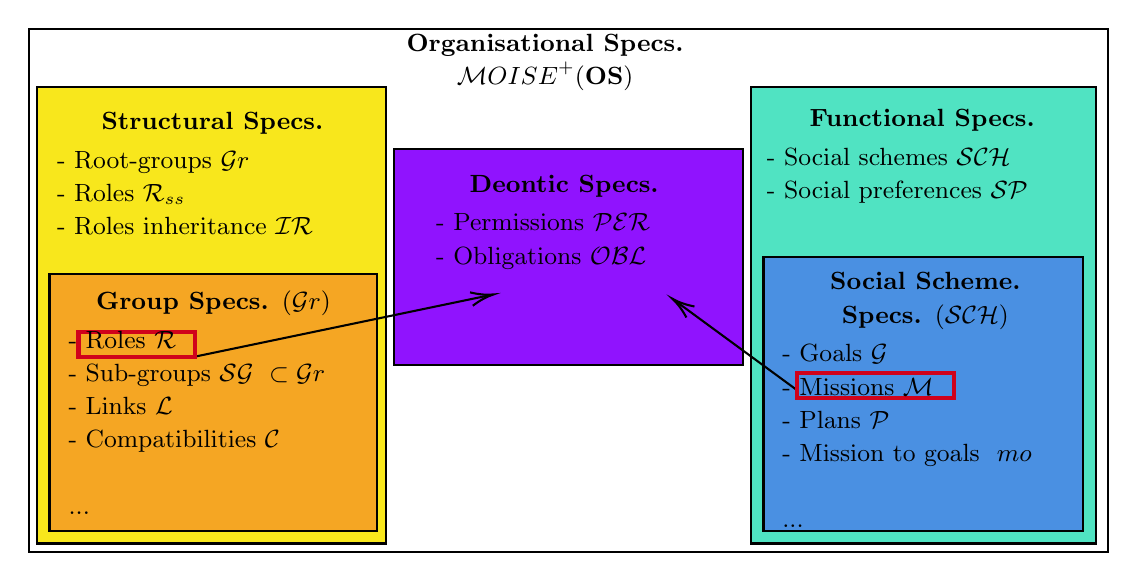
\begin{tikzpicture}[x=0.75pt,y=0.75pt,yscale=-1,xscale=1]
%uncomment if require: \path (0,1656); %set diagram left start at 0, and has height of 1656

%Shape: Rectangle [id:dp6756844921493015] 
\draw  [fill={rgb, 255:red, 248; green, 231; blue, 28 }  ,fill opacity=1 ] (46,1204) -- (214,1204) -- (214,1424) -- (46,1424) -- cycle ;
%Shape: Rectangle [id:dp3759944257810566] 
\draw  [fill={rgb, 255:red, 80; green, 227; blue, 194 }  ,fill opacity=1 ] (390,1204) -- (556,1204) -- (556,1424) -- (390,1424) -- cycle ;
%Shape: Rectangle [id:dp28244406216006945] 
\draw  [fill={rgb, 255:red, 144; green, 19; blue, 254 }  ,fill opacity=1 ] (218,1234) -- (386,1234) -- (386,1338) -- (218,1338) -- cycle ;
%Shape: Rectangle [id:dp32232123359581766] 
\draw   (42,1176) -- (562,1176) -- (562,1428) -- (42,1428) -- cycle ;
%Shape: Rectangle [id:dp7605706269262755] 
\draw  [fill={rgb, 255:red, 74; green, 144; blue, 226 }  ,fill opacity=1 ] (396,1286) -- (550,1286) -- (550,1418) -- (396,1418) -- cycle ;
%Shape: Rectangle [id:dp33110985390647496] 
\draw   (52,1294) -- (210,1294) -- (210,1418) -- (52,1418) -- cycle ;
%Shape: Rectangle [id:dp8653560038381976] 
\draw  [fill={rgb, 255:red, 245; green, 166; blue, 35 }  ,fill opacity=1 ] (52,1294) -- (210,1294) -- (210,1418) -- (52,1418) -- cycle ;
%Straight Lines [id:da09781093164567278] 
\draw    (412,1350) -- (353.61,1307.18) ;
\draw [shift={(352,1306)}, rotate = 36.25] [color={rgb, 255:red, 0; green, 0; blue, 0 }  ][line width=0.75]    (10.93,-3.29) .. controls (6.95,-1.4) and (3.31,-0.3) .. (0,0) .. controls (3.31,0.3) and (6.95,1.4) .. (10.93,3.29)   ;
%Straight Lines [id:da3938396723807833] 
\draw    (122,1334) -- (264.04,1304.41) ;
\draw [shift={(266,1304)}, rotate = 168.23] [color={rgb, 255:red, 0; green, 0; blue, 0 }  ][line width=0.75]    (10.93,-3.29) .. controls (6.95,-1.4) and (3.31,-0.3) .. (0,0) .. controls (3.31,0.3) and (6.95,1.4) .. (10.93,3.29)   ;
%Shape: Rectangle [id:dp269311335478327] 
\draw  [color={rgb, 255:red, 208; green, 2; blue, 27 }  ,draw opacity=1 ][line width=1.5]  (66,1322) -- (122,1322) -- (122,1334) -- (66,1334) -- cycle ;
%Shape: Rectangle [id:dp7449860119164387] 
\draw  [color={rgb, 255:red, 208; green, 2; blue, 27 }  ,draw opacity=1 ][line width=1.5]  (412,1342) -- (488,1342) -- (488,1354) -- (412,1354) -- cycle ;


% Text Node
\draw (472.5,1237.41) node   [align=left] {\begin{minipage}[lt]{112.2pt}\setlength\topsep{0pt}
\begin{center}
\textbf{{\small Functional Specs.}}
\end{center}
{\small  - Social schemes $\displaystyle \mathcal{SCH}$}\\{\small  - Social preferences $\displaystyle \mathcal{SP}$}
\end{minipage}};
% Text Node
\draw (474,1355) node   [align=left] {\begin{minipage}[lt]{103.36pt}\setlength\topsep{0pt}
\begin{center}
\textbf{{\small Social Scheme.}}\\{\small \textbf{Specs. }$\displaystyle (\mathcal{SCH})$}
\end{center}
{\small  - Goals $\displaystyle \mathcal{G}$}\\{\small  - Missions $\displaystyle \mathcal{M}$}\\{\small  - Plans $\displaystyle \mathcal{P}$}\\{\small  - Mission to goals \ $\displaystyle mo$}\\\\{\small  ...}
\end{minipage}};
% Text Node
\draw (131,1356) node   [align=left] {\begin{minipage}[lt]{104.72pt}\setlength\topsep{0pt}
\begin{center}
{\small \textbf{Group Specs. }$\displaystyle (\mathcal{G} r)$}
\end{center}
{\small  - Roles $\displaystyle \mathcal{R}$}\\{\small  - Sub-groups $\displaystyle \mathcal{SG} \ \subset \mathcal{G} r$}\\{\small  - Links $\displaystyle \mathcal{L}$}\\{\small  - Compatibilities $\displaystyle \mathcal{C}$}\\\\{\small  ...}
\end{minipage}};
% Text Node
\draw (181,1177) node [anchor=north west][inner sep=0.75pt]   [align=left] {\begin{minipage}[lt]{162.41pt}\setlength\topsep{0pt}
\begin{center}
{\small \textbf{Organisational Specs. }$\displaystyle \mathcal{M}\boldsymbol{OISE^{+}}$($\displaystyle \mathbf{OS}$)}
\end{center}

\end{minipage}};
% Text Node
\draw (300,1269.09) node   [align=left] {\begin{minipage}[lt]{92.48pt}\setlength\topsep{0pt}
\begin{center}
\textbf{{\small Deontic Specs.}}
\end{center}
{\small  - Permissions $\displaystyle \mathcal{PER}$}\\{\small  - Obligations $\displaystyle \mathcal{OBL}$}
\end{minipage}};
% Text Node
\draw (130.5,1245.69) node   [align=left] {\begin{minipage}[lt]{112.2pt}\setlength\topsep{0pt}
\begin{center}
\textbf{{\small Structural Specs.}}
\end{center}
{\small  - Root-groups $\displaystyle \mathcal{G} r$}\\{\small  - Roles $\displaystyle \mathcal{R}_{ss}$}\\{\small  - Roles inheritance $\displaystyle \mathcal{IR}$}
\end{minipage}};


\end{tikzpicture}
    \caption{Vue synthétique du modèle $\mathcal{M}OISE^+$}
    \label{fig:moise_model}
\end{figure}

Comme illustré dans \autoref{fig:moise_model}, $\mathcal{M}OISE^+$ comprend trois types de spécifications organisationnelles :

\noindent \paragraph{\textbf{Spécifications structurelles (SS)}} définissent la manière dont les agents sont structurés, exprimées sous la forme $\mathcal{SS} = \langle \mathcal{R}, \mathcal{IR}, \mathcal{G} \rangle$. $\mathcal{R}_{ss}$ est l'ensemble des rôles ($\rho \in \mathcal{R}$) avec une relation d'héritage $\mathcal{IR}$ où $\rho_1 \sqsubset \rho_2$ si $\rho_1$ hérite de $\rho_2$. $\mathcal{GR}$ comprend les groupes $\langle \mathcal{R}, \mathcal{SG}, \mathcal{L}^{intra}, \mathcal{L}^{inter}, \allowbreak \mathcal{C}^{intra}, \mathcal{C}^{inter}, np, ng \rangle$. Les liens ($\mathcal{L}$) définissent les connexions entre les rôles : connaissance, communication ou autorité. Les compatibilités $\mathcal{C}$ désignent les rôles que les agents peuvent jouer ensemble. Les liens et les compatibilités intra- et inter-groupes sont représentés par $\mathcal{L}^{intra}$, $\mathcal{L}^{inter}$, $\mathcal{C}^{intra}$ et $\mathcal{C}^{inter}$, où $np$ et $ng$ définissent le nombre de rôles et de sous-groupes.

\noindent \paragraph{\textbf{Spécifications fonctionnelles (FS)}} décrivent les objectifs des agents, représentés par $\mathcal{FS} = \langle \mathcal{SCH}, \mathcal{PO} \rangle$. Le schéma social $\mathcal{SCH}$ comprend les objectifs globaux $\mathcal{G}$, les missions $\mathcal{M}$ et les plans $\mathcal{P}$ qui organisent les objectifs dans une structure arborescente. Les plans relient les objectifs à un opérateur ($op$) indiquant la séquence, le choix ou l'achèvement parallèle. Les missions sont mappées à des ensembles d'objectifs ($mo$), et le nombre d'agents par mission est spécifié par $nm$. Les préférences $\mathcal{PO}$ indiquent les missions préférées des agents, notées $m_1 \prec m_2$.

\noindent \paragraph{\textbf{Spécifications déontiques (DS)}} indiquent la relation entre les rôles et les objectifs, donnée par $\mathcal{DS} = \langle \mathcal{OBL}, \mathcal{PER} \rangle$. Les contraintes temporelles $\mathcal{TC}$ fixent les périodes pour les autorisations ou les obligations ($Any$ pour n'importe quel moment). Les obligations ($\mathcal{OBL}$) exigent que les agents dans le rôle $\rho_a$ entreprennent la mission $m$ aux moments $tc$, tandis que les autorisations ($\mathcal{PER}$) le permettent. La fonction $rds$ mappe les rôles à leurs spécifications déontiques sous la forme $\langle tc, y, m \rangle$, où $y$ distingue l'autorisation (0) de l'obligation (1).

\

\noindent Les spécifications organisationnelles appliquées aux agents sont des rôles et des objectifs (sous forme de missions) via des autorisations ou des obligations. En effet, les autres spécifications structurelles telles que les compatibilités ou les liens sont inhérentes aux rôles. De même, nous considérons que les objectifs, les missions et leur mappage ($mo$) suffisent pour relier également toutes les autres spécifications fonctionnelles telles que les plans, les cardinalités ou les ordres de préférence.
Par conséquent, nous considérons qu'il suffit de prendre en compte les rôles, les missions (objectif et mappage) et les permissions/obligations pour relier $\mathcal{M}OISE^+$ à Dec-POMDP.


\begin{figure*}[t]

    \label{eq:single_value_function}
    \raggedright
    \textbf{\textit{Définition 1} \quad Fonction de valeur d'état adaptée aux \textbf{Guide de Contrainte} en mode AEC :}

    \begin{scriptsize}
        \vspace{-0.3cm}
        \begin{gather*}
            V^{\pi^j}(s_t) = \hspace{-0.75cm} \sum_{\textcolor{red}{ \substack{a_{t} \in A \text{ si } rn() < ch_{t}, \\
                        a_{t} \in A_{t} \text{ sinon}}
                }}{\hspace{-0.7cm} \pi_i(a_{t} | \omega_t)} \sum_{s_{t+1} \in S}{\hspace{-0.1cm} T(s_{t+1} | s_t, a_{t})\Bigl[R(s_t,a_{t},s_{t+1}) + \hspace{-0.1cm} \textcolor{blue}{ \sum_{m \in \mathcal{M}_i}{ \hspace{-0.1cm} v_m(t) \frac{grg_m(h_{t+1})}{1 - p + \epsilon} } } + \textcolor{red}{(1-ch_t) \times rrg(\omega_t,a_{t+1})} + V^{\pi^j_{i+1 \ mod \ n}}(s_{t+1})\Bigr]}
        \end{gather*}
        %
        \vspace{-0.3cm}
        %
        \textcolor{red}{$\hspace{0cm}\text{Avec } rag(h_t, \omega_t) = A_{t} \times \mathbb{R} \text{, } \langle a_t, ch_{t} \rangle \in A_{t} \times \mathbb{R} \text{ ; et } rn: \emptyset \to [0,1[ \text{, une fonction aléatoire uniforme}$}
        %
        \vspace{-0cm}
        \textcolor{blue}{
            \begin{gather*}
                \hspace{-4.1cm}\text{Avec } \omega_t = O(\omega_t | s_t, a_t) \text{ ; } h_t = \{h_0 = \langle \rangle, h_{t+1} = \langle h_t, \langle \omega_{t+1}, a_{t+1} \rangle \rangle \} \text{ ; } grg_m(h) = \hspace{-0.8cm} \sum_{(grg_i,w_i) \in mo(m)}{\hspace{-0.8cm} w_i \times grg_i(h)} \text{ ; } \epsilon \in \mathbb{R}_{>0} \text{ ; }
            \end{gather*}
        }
        \vspace{-1.05cm}
        \textcolor{blue}{
            \begin{gather*}
                \hspace{-8.5cm}
                v_m(t) = \{ 1 \text{ si } t \in t_c \text{ ; sinon } 0 \} \text{ ; et } \mathcal{M}_i = \{m_j \mid \langle ar(i),m_j,t_c,p \rangle \in \mathcal{M}\}
            \end{gather*}
        }
        \vspace{-0.6cm}

    \end{scriptsize}

\end{figure*}


\subsection{Lien entre $\mathcal{M}OISE^+$ et MARL}

\begin{figure}[h!]
    \centering
    \tikzset{every picture/.style={line width=0.75pt}} %set default line width to 0.75pt        

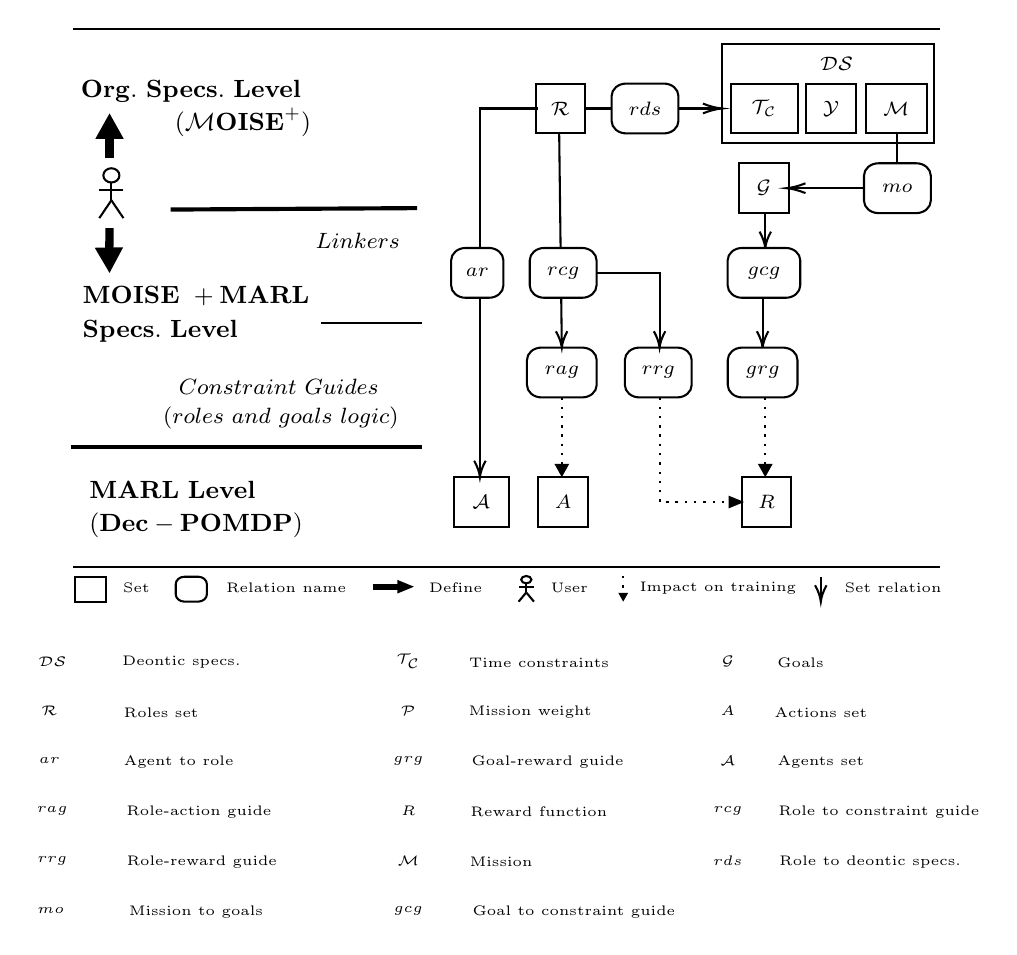
\begin{tikzpicture}[x=0.75pt,y=0.75pt,yscale=-1.2,xscale=1.4]
    %uncomment if require: \path (0,2584); %set diagram left start at 0, and has height of 2584

    %Straight Lines [id:da4973066741986565] 
    \draw [line width=1.5]    (118.21,2302.58) -- (203.1,2302) ;
    %Straight Lines [id:da14807114776731778] 
    \draw    (368.35,2272) -- (368.35,2294) -- (332.16,2294) ;
    \draw [shift={(330.16,2294)}, rotate = 360] [color={rgb, 255:red, 0; green, 0; blue, 0 }  ][line width=0.75]    (6.56,-1.97) .. controls (4.17,-0.84) and (1.99,-0.18) .. (0,0) .. controls (1.99,0.18) and (4.17,0.84) .. (6.56,1.97)   ;
    %Straight Lines [id:da16285043353898754] 
    \draw [line width=1.5]    (83.88,2398) -- (204.61,2398) ;
    %Straight Lines [id:da6299512000169913] 
    \draw    (169.94,2348) -- (204.61,2348) ;
    %Straight Lines [id:da64750232417664] 
    \draw    (84.65,2446) -- (383.15,2446) ;
    %Straight Lines [id:da35895220906699743] 
    \draw    (84.65,2230) -- (383,2230) ;
    %Straight Lines [id:da715014372569708] 
    \draw    (244.68,2262) -- (224.68,2262) -- (224.68,2408) ;
    \draw [shift={(224.68,2410)}, rotate = 270] [color={rgb, 255:red, 0; green, 0; blue, 0 }  ][line width=0.75]    (6.56,-1.97) .. controls (4.17,-0.84) and (1.99,-0.18) .. (0,0) .. controls (1.99,0.18) and (4.17,0.84) .. (6.56,1.97)   ;
    %Straight Lines [id:da71870438525014] 
    \draw    (251.96,2328) -- (286.51,2328) -- (286.51,2356) ;
    \draw [shift={(286.51,2358)}, rotate = 270] [color={rgb, 255:red, 0; green, 0; blue, 0 }  ][line width=0.75]    (6.56,-1.97) .. controls (4.17,-0.84) and (1.99,-0.18) .. (0,0) .. controls (1.99,0.18) and (4.17,0.84) .. (6.56,1.97)   ;
    %Straight Lines [id:da6006267784187092] 
    \draw [line width=0.75]  [dash pattern={on 0.84pt off 2.51pt}]  (252.87,2378) -- (252.87,2407) ;
    \draw [shift={(252.87,2410)}, rotate = 270] [fill={rgb, 255:red, 0; green, 0; blue, 0 }  ][line width=0.08]  [draw opacity=0] (5.36,-2.57) -- (0,0) -- (5.36,2.57) -- cycle    ;
    %Straight Lines [id:da8743336135156266] 
    \draw    (322.88,2304) -- (322.88,2316) ;
    \draw [shift={(322.88,2318)}, rotate = 270] [color={rgb, 255:red, 0; green, 0; blue, 0 }  ][line width=0.75]    (6.56,-1.97) .. controls (4.17,-0.84) and (1.99,-0.18) .. (0,0) .. controls (1.99,0.18) and (4.17,0.84) .. (6.56,1.97)   ;
    %Straight Lines [id:da14641229967966152] 
    \draw [line width=0.75]  [dash pattern={on 0.84pt off 2.51pt}]  (322.88,2378) -- (322.88,2407) ;
    \draw [shift={(322.88,2410)}, rotate = 270] [fill={rgb, 255:red, 0; green, 0; blue, 0 }  ][line width=0.08]  [draw opacity=0] (5.36,-2.57) -- (0,0) -- (5.36,2.57) -- cycle    ;
    %Straight Lines [id:da9260929933425808] 
    \draw [line width=0.75]  [dash pattern={on 0.84pt off 2.51pt}]  (286.51,2378) -- (286.51,2420) -- (312.61,2420) ;
    \draw [shift={(315.61,2420)}, rotate = 180] [fill={rgb, 255:red, 0; green, 0; blue, 0 }  ][line width=0.08]  [draw opacity=0] (5.36,-2.57) -- (0,0) -- (5.36,2.57) -- cycle    ;
    %Straight Lines [id:da3057006030233673] 
    \draw [line width=0.75]  [dash pattern={on 0.84pt off 2.51pt}]  (274,2449.7) -- (274,2457) ;
    \draw [shift={(274,2460)}, rotate = 270] [fill={rgb, 255:red, 0; green, 0; blue, 0 }  ][line width=0.08]  [draw opacity=0] (3.57,-1.72) -- (0,0) -- (3.57,1.72) -- cycle    ;
    %Straight Lines [id:da07288166228322246] 
    \draw    (342,2449.98) -- (342,2458) ;
    \draw [shift={(342,2460)}, rotate = 270] [color={rgb, 255:red, 0; green, 0; blue, 0 }  ][line width=0.75]    (6.56,-1.97) .. controls (4.17,-0.84) and (1.99,-0.18) .. (0,0) .. controls (1.99,0.18) and (4.17,0.84) .. (6.56,1.97)   ;
    %Shape: Ellipse [id:dp8508274348425935] 
    \draw   (95.09,2288.86) .. controls (95.09,2287.28) and (96.33,2286) .. (97.85,2286) .. controls (99.38,2286) and (100.62,2287.28) .. (100.62,2288.86) .. controls (100.62,2290.44) and (99.38,2291.71) .. (97.85,2291.71) .. controls (96.33,2291.71) and (95.09,2290.44) .. (95.09,2288.86) -- cycle ;
    %Straight Lines [id:da3825450168053828] 
    \draw    (97.85,2291.71) -- (97.85,2298.86) ;
    %Straight Lines [id:da521321206042058] 
    \draw    (97.85,2298.86) -- (93.71,2306) ;
    %Straight Lines [id:da055514206493922025] 
    \draw    (97.85,2298.86) -- (102,2306) ;
    %Straight Lines [id:da8996496708356774] 
    \draw    (102,2294.57) -- (93.71,2294.57) ;

    %Straight Lines [id:da31678488015771755] 
    \draw [line width=2.25]    (188,2454) -- (196.97,2454) ;
    \draw [shift={(201.97,2454)}, rotate = 180] [fill={rgb, 255:red, 0; green, 0; blue, 0 }  ][line width=0.08]  [draw opacity=0] (5.72,-2.75) -- (0,0) -- (5.72,2.75) -- cycle    ;
    %Shape: Ellipse [id:dp3927356466672782] 
    \draw   (238.88,2451.17) .. controls (238.88,2450.36) and (239.67,2449.7) .. (240.64,2449.7) .. controls (241.61,2449.7) and (242.4,2450.36) .. (242.4,2451.17) .. controls (242.4,2451.99) and (241.61,2452.65) .. (240.64,2452.65) .. controls (239.67,2452.65) and (238.88,2451.99) .. (238.88,2451.17) -- cycle ;
    %Straight Lines [id:da3365602555559104] 
    \draw    (240.64,2452.65) -- (240.64,2456.32) ;
    %Straight Lines [id:da7990875235744026] 
    \draw    (240.64,2456.32) -- (238,2460) ;
    %Straight Lines [id:da23945649338821617] 
    \draw    (240.64,2456.32) -- (243.28,2460) ;
    %Straight Lines [id:da11927353559661591] 
    \draw    (243.28,2454.12) -- (238,2454.12) ;

    %Straight Lines [id:da5816423191130675] 
    \draw    (251.96,2272) -- (252.85,2356) ;
    \draw [shift={(252.87,2358)}, rotate = 269.39] [color={rgb, 255:red, 0; green, 0; blue, 0 }  ][line width=0.75]    (6.56,-1.97) .. controls (4.17,-0.84) and (1.99,-0.18) .. (0,0) .. controls (1.99,0.18) and (4.17,0.84) .. (6.56,1.97)   ;
    %Straight Lines [id:da9310455126832857] 
    \draw    (321.97,2338) -- (321.97,2356) ;
    \draw [shift={(321.97,2358)}, rotate = 270] [color={rgb, 255:red, 0; green, 0; blue, 0 }  ][line width=0.75]    (6.56,-1.97) .. controls (4.17,-0.84) and (1.99,-0.18) .. (0,0) .. controls (1.99,0.18) and (4.17,0.84) .. (6.56,1.97)   ;
    %Shape: Rectangle [id:dp293492578719597] 
    \draw   (120,2453) .. controls (120,2451.34) and (121.34,2450) .. (123,2450) -- (127.72,2450) .. controls (129.37,2450) and (130.72,2451.34) .. (130.72,2453) -- (130.72,2457) .. controls (130.72,2458.66) and (129.37,2460) .. (127.72,2460) -- (123,2460) .. controls (121.34,2460) and (120,2458.66) .. (120,2457) -- cycle ;
    %Straight Lines [id:da33566712615128225] 
    \draw    (261.05,2262) -- (306,2262) ;
    \draw [shift={(308,2262)}, rotate = 180] [color={rgb, 255:red, 0; green, 0; blue, 0 }  ][line width=0.75]    (6.56,-1.97) .. controls (4.17,-0.84) and (1.99,-0.18) .. (0,0) .. controls (1.99,0.18) and (4.17,0.84) .. (6.56,1.97)   ;
    %Shape: Rectangle [id:dp28383270948937667] 
    \draw   (308,2236) -- (381.08,2236) -- (381.08,2276) -- (308,2276) -- cycle ;
    %Straight Lines [id:da18020989903965012] 
    \draw [line width=3]    (97.22,2282) -- (97.22,2270) ;
    \draw [shift={(97.22,2264)}, rotate = 90] [fill={rgb, 255:red, 0; green, 0; blue, 0 }  ][line width=0.08]  [draw opacity=0] (10.18,-4.89) -- (0,0) -- (10.18,4.89) -- cycle    ;
    %Straight Lines [id:da018421338049046554] 
    \draw [line width=3]    (97.22,2310) -- (97.11,2322.37) ;
    \draw [shift={(97.22,2328)}, rotate = 268.86] [fill={rgb, 255:red, 0; green, 0; blue, 0 }  ][line width=0.08]  [draw opacity=0] (10.18,-4.89) -- (0,0) -- (10.18,4.89) -- cycle    ;
    %Shape: Rectangle [id:dp7281037051878541] 
    \draw   (85.42,2450) -- (96.13,2450) -- (96.13,2460) -- (85.42,2460) -- cycle ;

    % Text Node
    \draw (362,2544.5) node  [font=\tiny] [align=left] {Role to constraint guide};
    % Text Node
    \draw (342,2524.5) node  [font=\tiny] [align=left] {Agents set};
    % Text Node
    \draw (342,2504.5) node  [font=\tiny] [align=left] {Actions set};
    % Text Node
    \draw (257,2584.5) node  [font=\tiny] [align=left] {Goal to constraint guide};
    % Text Node
    \draw (335,2484.5) node  [font=\tiny] [align=left] {Goals};
    % Text Node
    \draw (359,2564.5) node  [font=\tiny] [align=left] {Role to deontic specs.};
    % Text Node
    \draw (232,2564.5) node  [font=\tiny] [align=left] {Mission};
    % Text Node
    \draw (245,2544.5) node  [font=\tiny] [align=left] {Reward function};
    % Text Node
    \draw (248,2524.5) node  [font=\tiny] [align=left] {Goal-reward guide};
    % Text Node
    \draw (242,2504.5) node  [font=\tiny] [align=left] {Mission weight};
    % Text Node
    \draw (245,2484.5) node  [font=\tiny] [align=left] {Time constraints};
    % Text Node
    \draw (127,2584.5) node  [font=\tiny] [align=left] {Mission to goals};
    % Text Node
    \draw (129,2564.5) node  [font=\tiny] [align=left] {Role-reward guide};
    % Text Node
    \draw (128,2544.5) node  [font=\tiny] [align=left] {Role-action guide};
    % Text Node
    \draw (121,2524.5) node  [font=\tiny] [align=left] {Agent to role};
    % Text Node
    \draw (115,2504.5) node  [font=\tiny] [align=left] {Roles set};
    % Text Node
    \draw (122,2484.5) node  [font=\tiny] [align=left] {Deontic specs.};
    % Text Node
    \draw (310,2544) node  [font=\tiny] [align=left] {$\displaystyle \boldsymbol{rcg}$};
    % Text Node
    \draw (200,2504) node  [font=\tiny] [align=left] {$\displaystyle \mathcal{P}$};
    % Text Node
    \draw (200,2484) node  [font=\tiny] [align=left] {$\displaystyle \mathcal{T_{C}}$};
    % Text Node
    \draw (200,2564) node  [font=\tiny] [align=left] {$\displaystyle \mathcal{M}$};
    % Text Node
    \draw (77.5,2484) node  [font=\tiny] [align=left] {$\displaystyle \mathcal{DS}$};
    % Text Node
    \draw (310,2564) node  [font=\tiny] [align=left] {$\displaystyle \boldsymbol{rds}$};
    % Text Node
    \draw (310,2504) node  [font=\tiny] [align=left] {$\displaystyle \boldsymbol{A}$};
    % Text Node
    \draw (200,2544) node  [font=\tiny] [align=left] {$\displaystyle \boldsymbol{R}$};
    % Text Node
    \draw (310,2524) node  [font=\tiny] [align=left] {$\displaystyle \mathcal{A}$};
    % Text Node
    \draw (200,2524) node  [font=\tiny] [align=left] {$\displaystyle \boldsymbol{grg}$};
    % Text Node
    \draw (77.5,2564) node  [font=\tiny] [align=left] {$\displaystyle \boldsymbol{rrg}$};
    % Text Node
    \draw (77.5,2544) node  [font=\tiny] [align=left] {$\displaystyle \boldsymbol{rag}$};
    % Text Node
    \draw (200,2584) node  [font=\tiny] [align=left] {$\displaystyle \boldsymbol{gcg}$};
    % Text Node
    \draw (76.5,2524) node  [font=\tiny] [align=left] {$\displaystyle \boldsymbol{ar}$};
    % Text Node
    \draw (77,2584) node  [font=\tiny] [align=left] {$\displaystyle \boldsymbol{mo}$};
    % Text Node
    \draw (76.5,2504) node  [font=\tiny] [align=left] {$\displaystyle \mathcal{R}$};
    % Text Node
    \draw (310,2484) node  [font=\tiny] [align=left] {$\displaystyle \mathcal{G}$};


    % Text Node
    \draw  [fill={rgb, 255:red, 255; green, 255; blue, 255 }  ,fill opacity=1 ]  (241.82,2323) .. controls (241.82,2320.24) and (244.06,2318) .. (246.82,2318) -- (259.82,2318) .. controls (262.58,2318) and (264.82,2320.24) .. (264.82,2323) -- (264.82,2333) .. controls (264.82,2335.76) and (262.58,2338) .. (259.82,2338) -- (246.82,2338) .. controls (244.06,2338) and (241.82,2335.76) .. (241.82,2333) -- cycle  ;
    \draw (253.32,2328) node  [font=\scriptsize] [align=left] {$\displaystyle \boldsymbol{rcg}$};
    % Text Node
    \draw    (337,2252) -- (354,2252) -- (354,2272) -- (337,2272) -- cycle  ;
    \draw (345.5,2262) node  [font=\scriptsize] [align=left] {$\displaystyle \mathcal{Y}$};
    % Text Node
    \draw    (311,2252) -- (334,2252) -- (334,2272) -- (311,2272) -- cycle  ;
    \draw (322.5,2262) node  [font=\scriptsize] [align=left] {$\displaystyle \mathcal{T_{C}}$};
    % Text Node
    \draw    (357.39,2252) -- (378.39,2252) -- (378.39,2272) -- (357.39,2272) -- cycle  ;
    \draw (367.89,2262) node  [font=\scriptsize] [align=left] {$\displaystyle \mathcal{M}$};
    % Text Node
    \draw (347.43,2244) node  [font=\scriptsize] [align=left] {$\displaystyle \mathcal{DS}$};
    % Text Node
    \draw  [fill={rgb, 255:red, 255; green, 255; blue, 255 }  ,fill opacity=1 ]  (270,2257) .. controls (270,2254.24) and (272.24,2252) .. (275,2252) -- (288,2252) .. controls (290.76,2252) and (293,2254.24) .. (293,2257) -- (293,2267) .. controls (293,2269.76) and (290.76,2272) .. (288,2272) -- (275,2272) .. controls (272.24,2272) and (270,2269.76) .. (270,2267) -- cycle  ;
    \draw (281.5,2262) node  [font=\scriptsize] [align=left] {$\displaystyle \boldsymbol{rds}$};
    % Text Node
    \draw (158,2454.5) node  [font=\tiny] [align=left] {Relation name};
    % Text Node
    \draw (106.46,2454.5) node  [font=\tiny] [align=left] {Set};
    % Text Node
    \draw (255.47,2454.5) node  [font=\tiny] [align=left] {User};
    % Text Node
    \draw (216.32,2454.5) node  [font=\tiny] [align=left] {Define};
    % Text Node
    \draw (366.91,2454.5) node  [font=\tiny] [align=left] {Set relation};
    % Text Node
    \draw (306.61,2454.5) node  [font=\tiny] [align=left] {Impact on training};
    % Text Node
    \draw    (244.82,2410) -- (261.82,2410) -- (261.82,2430) -- (244.82,2430) -- cycle  ;
    \draw (253.32,2420) node  [font=\scriptsize] [align=left] {$\displaystyle \boldsymbol{A}$};
    % Text Node
    \draw    (314.84,2410) -- (331.84,2410) -- (331.84,2430) -- (314.84,2430) -- cycle  ;
    \draw (323.34,2420) node  [font=\scriptsize] [align=left] {$\displaystyle \boldsymbol{R}$};
    % Text Node
    \draw    (215.63,2410) -- (234.63,2410) -- (234.63,2430) -- (215.63,2430) -- cycle  ;
    \draw (225.13,2420) node  [font=\scriptsize] [align=left] {$\displaystyle \mathcal{A}$};
    % Text Node
    \draw  [fill={rgb, 255:red, 255; green, 255; blue, 255 }  ,fill opacity=1 ]  (309.97,2363) .. controls (309.97,2360.24) and (312.21,2358) .. (314.97,2358) -- (328.97,2358) .. controls (331.73,2358) and (333.97,2360.24) .. (333.97,2363) -- (333.97,2373) .. controls (333.97,2375.76) and (331.73,2378) .. (328.97,2378) -- (314.97,2378) .. controls (312.21,2378) and (309.97,2375.76) .. (309.97,2373) -- cycle  ;
    \draw (321.97,2368) node  [font=\scriptsize] [align=left] {$\displaystyle \boldsymbol{grg}$};
    % Text Node
    \draw    (274.56,2363) .. controls (274.56,2360.24) and (276.8,2358) .. (279.56,2358) -- (292.56,2358) .. controls (295.32,2358) and (297.56,2360.24) .. (297.56,2363) -- (297.56,2373) .. controls (297.56,2375.76) and (295.32,2378) .. (292.56,2378) -- (279.56,2378) .. controls (276.8,2378) and (274.56,2375.76) .. (274.56,2373) -- cycle  ;
    \draw (286.06,2368) node  [font=\scriptsize] [align=left] {$\displaystyle \boldsymbol{rrg}$};
    % Text Node
    \draw    (240.87,2363) .. controls (240.87,2360.24) and (243.11,2358) .. (245.87,2358) -- (259.87,2358) .. controls (262.63,2358) and (264.87,2360.24) .. (264.87,2363) -- (264.87,2373) .. controls (264.87,2375.76) and (262.63,2378) .. (259.87,2378) -- (245.87,2378) .. controls (243.11,2378) and (240.87,2375.76) .. (240.87,2373) -- cycle  ;
    \draw (252.87,2368) node  [font=\scriptsize] [align=left] {$\displaystyle \boldsymbol{rag}$};
    % Text Node
    \draw (156.15,2380.5) node  [font=\footnotesize] [align=left] {$\displaystyle  \begin{array}{{>{\displaystyle}l}}
                \ \ \boldsymbol{Constraint\ Guides} \\
                ( roles\ and\ goals\ logic)
            \end{array}$};
    % Text Node
    \draw  [fill={rgb, 255:red, 255; green, 255; blue, 255 }  ,fill opacity=1 ]  (309.93,2323) .. controls (309.93,2320.24) and (312.17,2318) .. (314.93,2318) -- (329.93,2318) .. controls (332.69,2318) and (334.93,2320.24) .. (334.93,2323) -- (334.93,2333) .. controls (334.93,2335.76) and (332.69,2338) .. (329.93,2338) -- (314.93,2338) .. controls (312.17,2338) and (309.93,2335.76) .. (309.93,2333) -- cycle  ;
    \draw (322.43,2328) node  [font=\scriptsize] [align=left] {$\displaystyle \boldsymbol{gcg}$};
    % Text Node
    \draw  [fill={rgb, 255:red, 255; green, 255; blue, 255 }  ,fill opacity=1 ]  (214.77,2323) .. controls (214.77,2320.24) and (217.01,2318) .. (219.77,2318) -- (227.77,2318) .. controls (230.53,2318) and (232.77,2320.24) .. (232.77,2323) -- (232.77,2333) .. controls (232.77,2335.76) and (230.53,2338) .. (227.77,2338) -- (219.77,2338) .. controls (217.01,2338) and (214.77,2335.76) .. (214.77,2333) -- cycle  ;
    \draw (223.77,2328) node  [font=\scriptsize] [align=left] {$\displaystyle \boldsymbol{ar}$};
    % Text Node
    \draw  [fill={rgb, 255:red, 255; green, 255; blue, 255 }  ,fill opacity=1 ]  (356.85,2289) .. controls (356.85,2286.24) and (359.08,2284) .. (361.85,2284) -- (374.85,2284) .. controls (377.61,2284) and (379.85,2286.24) .. (379.85,2289) -- (379.85,2299) .. controls (379.85,2301.76) and (377.61,2304) .. (374.85,2304) -- (361.85,2304) .. controls (359.08,2304) and (356.85,2301.76) .. (356.85,2299) -- cycle  ;
    \draw (368.35,2294) node  [font=\scriptsize] [align=left] {$\displaystyle \boldsymbol{mo}$};
    % Text Node
    \draw (127,2344.5) node  [font=\small] [align=left] {$\displaystyle  \begin{array}{{>{\displaystyle}l}}
                \mathbf{MOISE\ +MARL} \\
                \mathbf{Specs.\ Level}
            \end{array}$};
    % Text Node
    \draw (127,2422.5) node  [font=\small] [align=left] {$\displaystyle  \begin{array}{{>{\displaystyle}l}}
                \mathbf{MARL\ Level} \\
                \mathbf{(Dec-POMDP)}
            \end{array}$};
    % Text Node
    \draw    (243.91,2252) -- (260.91,2252) -- (260.91,2272) -- (243.91,2272) -- cycle  ;
    \draw (252.41,2262) node  [font=\scriptsize] [align=left] {$\displaystyle \mathcal{R}$};
    % Text Node
    \draw (182.64,2315) node  [font=\footnotesize] [align=left] {$\displaystyle \boldsymbol{Linkers}$};
    % Text Node
    \draw    (313.93,2284) -- (330.93,2284) -- (330.93,2304) -- (313.93,2304) -- cycle  ;
    \draw (322.43,2294) node  [font=\scriptsize] [align=left] {$\displaystyle \mathcal{G}$};
    % Text Node
    \draw (127,2261.5) node  [font=\small] [align=left] {$\displaystyle  \begin{array}{{>{\displaystyle}l}}
                \mathbf{{\displaystyle Org.\ Specs.\ Level}} \\
                {\displaystyle \ \ \ \ \ \ \ \ \ \ \ (\mathcal{M}\mathbf{OISE^+})}
            \end{array}$};


\end{tikzpicture}
    \caption{Une vue minimale du cadre MOISE+MARL :
        Les utilisateurs définissent d'abord les spécifications $\mathcal{M}OISE^+$, qui comprennent les rôles ($\mathcal{R}$) et les missions ($\mathcal{M}$), tous deux associés via $rds$. Ils créent ensuite les spécifications MOISE+MARL en définissant d'abord des \textbf{guides de contraintes} tels que $rag$ et $rrg$ pour spécifier la logique des rôles, et $grg$ pour la logique des objectifs.
        Ensuite, des \textbf{Linkers} sont utilisés pour connecter les agents aux rôles via $ar$ et pour relier la logique des guides de contraintes aux spécifications $\mathcal{M}OISE^+$ définies. Une fois cette configuration effectuée, les rôles peuvent être attribués aux agents et le cadre MARL se met à jour en conséquence pendant la formation.
    }
    \label{fig:mm_synthesis}
\end{figure}

Nous avons identifié les modèles organisationnels \textit{AGR}~\cite{ferber2003} (Agent Group Role) et $\mathcal{M}OISE^+$~\cite{Hubner2007}. Contrairement à l'AGR, qui est un cadre informel introduisant des rôles en fonction des groupes, $\mathcal{M}OISE^+$ fournit une description plus détaillée et plus flexible des structures et des fonctions d'un MAS, facilitant ainsi la description formelle des politiques des agents dans le MARL.

\

\noindent Les \textbf{guides de contraintes} sont trois nouvelles relations introduites pour décrire la logique des rôles et des objectifs de $\mathcal{M}OISE^+$ dans le formalisme Dec-POMDP :
%
% \begin{itemize}
\begin{enumerate*}[label={\roman*) },itemjoin={; \quad}]

    \item \textbf{Guide d'action des rôles} \quad $rag : H \times \Omega \rightarrow \mathcal{P}(A \times \mathbb{R})$, la relation qui modélise un rôle comme un ensemble de règles qui, pour chaque paire constituée d'un historique $h \in H$ et d'une observation reçue par l'agent $\omega \in \Omega$, associe des actions attendues $A \in \mathcal{P}(A)$ chacune associée à une contrainte de difficulté $ch \in [0,1]$ ($ch = 1$ par défaut). En limitant le choix de l'action suivante parmi celles autorisées, l'agent est contraint d'adhérer au comportement attendu du rôle
    \item \textbf{Guide de récompense des rôles} \quad $rrg: H \times \Omega \times A \to \mathbb{R} = \{r_m \text{ si } a \notin A_\omega \text{, } rag(h, \omega) \allowbreak = \allowbreak A_\omega \times \mathbb{R} \text{, } h \in H; \text{ sinon } 0\}$, la relation qui modélise un rôle en ajoutant une pénalité $r_m$ à la récompense globale si la dernière action choisie par l'agent $a \in A$ n'est pas autorisée. Cela vise à encourager l'agent à respecter le comportement attendu d'un rôle
    \item \textbf{Guide de récompense d'objectif} \quad $grg: H \rightarrow \mathbb{R}$, la relation qui modélise un objectif comme une contrainte souple en ajoutant un bonus $r_b \in \mathbb{R}$ à la récompense globale si l'historique de l'agent $h \in H$ contient une sous-séquence caractéristique $h_g \in H_g$ de l'objectif, encourageant ainsi l'agent à l'atteindre.
\end{enumerate*}
% \end{itemize}

\

\noindent Enfin, nous introduisons les \textbf{Linkers} pour relier les spécifications organisationnelles $\mathcal{M}OISE^+$ aux guides de contraintes et aux agents :
%
% \begin{itemize}
\begin{enumerate*}[label={\roman*) },itemjoin={; \quad}]

    \item \textbf{Agent à rôle} \quad $ar : \mathcal{A} \to \mathcal{R}$, relation bijective reliant un agent à un rôle ;
    \item \textbf{Guide rôle-contrainte} \quad $rcg: \mathcal{R} \rightarrow rag \cup rrg$, la relation associant chaque rôle $\mathcal{M}OISE^+$ à une relation $rag$ ou $rrg$, forçant/encourageant l'agent à suivre les actions attendues pour le rôle $\rho \in \mathcal{R}$ ;
    \item \textbf{Guide objectif-contrainte} \quad $gcg : \mathcal{G} \rightarrow grg$, la relation reliant les objectifs aux relations $grg$, représentant les objectifs comme des récompenses dans MARL.
\end{enumerate*}
% \end{itemize}

\paragraph{\textbf{Résolution du problème MOISE+MARL}}
% formalisé comme $MM = \langle D, \mathcal{OS}\allowbreak, ar, rcg, \allowbreak gcg, rag, rrg, grg\rangle$
implique de trouver une politique conjointe $\pi^{j} = \{\pi^j_0,\pi^j_1\dots\pi^j_n\}$ qui maximise la fonction de valeur d'état $V^{\pi^{j}}$ (ou atteint un seuil minimal), qui représente la récompense cumulative attendue à partir d'un état initial $s \in S$ et en suivant la politique conjointe $\pi^{j}$, en appliquant des actions conjointes successives $a^{j} \in A^n$ sous des contraintes supplémentaires. La valeur d'état est décrite dans le cas où les agents agissent de manière séquentielle et cyclique (mode Agent Environment Cycle - AEC) dans \hyperref[eq:single_value_function]{Définition 1}, en adaptant sa définition pour les rôles (en rouge) et les missions (en bleu), ce qui a un impact sur l'espace d'action et la récompense. \autoref{fig:mm_synthesis} illustre les liens entre $\mathcal{M}OISE^+$ et Dec-POMDP via le cadre MOISE+MARL.

À tout moment $t \in \mathbb{N}$ (initialement $t = 0$), l'agent $i = t \ mod \ n$ est contraint à un rôle $\rho_i = ar(i)$. Pour chaque spécification déontique valide dans le temps $d_i = rds(\rho_i) = \langle tc_i,y_i, m_i \rangle$, l'agent est autorisé (si $y_i = 0$) ou obligé (si $y_i = 1$) de s'engager dans la mission $m_i \in \mathcal{M}, \mathcal{G}_{m_i} = mo(m_i)$, et $n \in \mathbb{N}$ le nombre d'agents.
%
Tout d'abord, sur la base de l'observation reçue $\omega_t$, l'agent doit choisir une action soit parmi les actions attendues du rôle $A_t$ si une valeur aléatoire est inférieure à la contrainte de rigidité du rôle $ch_t$, soit parmi l'ensemble de toutes les actions $A$ dans le cas contraire. Si $ch_t = 1$, le rôle est fortement contraignant pour l'agent et faiblement contraignant dans le cas contraire.
%
Ensuite, l'action est appliquée à l'état actuel $s_t$ pour passer à l'état suivant $s_{t+1}$, générer l'observation suivante $\omega_{t+1}$ et produire une récompense. La récompense est la somme de la récompense globale avec les pénalités et les bonus obtenus à partir des spécifications organisationnelles : \quad i) la somme des bonus pour les objectifs associés à chaque mission temporairement valide (via les guides de récompense des objectifs), pondérée par la valeur associée ($\frac{1}{1-p+\epsilon}$) ; \quad ii) la pénalité associée au rôle (via les « guides de récompense des rôles ») pondérée par la rigidité de la contrainte de rôle.
%
Enfin, le calcul de la récompense cumulative se poursuit dans l'état suivant $s_{t+1} \in S$ avec l'agent suivant $(i+1) \ mod \ n$.

\subsection{Faciliter la mise en œuvre des guides de contraintes}

Les rôles, les objectifs et les missions étant de simples étiquettes, leur définition est supposée. Cependant, la mise en œuvre d'une relation $rag$, $rrg$ ou $grg$ nécessite de définir un nombre potentiellement important d'historiques, qui peuvent être redondants. Par conséquent, une définition extensionnelle d'un ensemble d'histoires peut s'avérer fastidieuse. De plus, la logique de tous les guides de contraintes prend la trajectoire de l'agent comme entrée pour déterminer si la trajectoire appartient à un ensemble d'histoires prédéfini. Par exemple, une relation $rag$ peut être considérée comme déterminant les prochaines actions attendues en fonction de l'appartenance de la trajectoire à un ensemble donné et de la nouvelle observation reçue.

Une première approche consiste à laisser les utilisateurs développer leurs guides de contraintes de manière intensive avec une logique personnalisée (telle qu'un code script) afin d'analyser l'historique et de calculer le résultat de manière gérable. Dans ce cas, la relation $b_g: H \to \{0,1\}$ formalise la manière dont les utilisateurs proposent de déterminer si un historique appartient à un ensemble prédéfini $H_g$.
Pour aider à mettre en œuvre cette relation, nous proposons un \textbf{modèle basé sur la trajectoire} (TP) inspiré du traitement du langage naturel, noté $p \in P$, comme moyen de définir un ensemble d'historiques de manière intensive.

Un TP implique que toute observation ou action réelle considérée est connue et mappée à une étiquette $l \in L$ (via $l: \Omega \cup A \to L$) afin d'être facilement gérée. Un TP $p \in P$ est défini comme suit : $p$ est : soit une « séquence feuille » désignée par un couple d'histoire-cardinalité $s_l = \langle h, \{c_min,c_max\}\rangle$ (où $h \in H, c_{min} \in \mathbb{N}, c_{max} \in \mathbb{N} \cup "*")$ ; soit une « séquence de nœuds » désignée par un couple constitué d'un tuple de séquences concrètes et d'une cardinalité $s_n = \langle \langle s_{l_1}, s_{l_1}\dots \rangle, \{c_min,c_max\}\rangle$. Par exemple, le motif $p = \allowbreak "[o_1,a_1,[o_2,a_2]\langle0,2\rangle]\langle1,*\rangle"$ peut être formalisé comme la séquence de nœuds $\allowbreak \langle \langle \langle o_1,a_1\rangle,\langle 1,1 \rangle \rangle, \langle \langle o_2,a_2 \rangle, \langle 0,2 \rangle \rangle \rangle \langle 1,"*" \rangle$, indiquant l'ensemble des historiques $H_p$ contenant au moins une fois la sous-séquence composée d'une première paire $\langle o_1,a_1\rangle$ puis au plus deux répétitions de la paire $\langle o_2,a_2 \rangle$.
La relation $b_g$ devient alors $b_g(h) = m(p_g,h), \text{ avec } m: P \times H \to \{0,1\}$ indiquant si une histoire $h \in H$ correspond à un modèle d'histoire $p \in P$ décrivant un ensemble d'histoires $H_g$.

\section{La méthode TEMM}
\label{sec:TEMM_algorithm}

Comme présenté dans \autoref{sec:related_works}, nous n'avons pas pu identifier de méthode disponible qui réponde pleinement à nos exigences en matière de détermination des rôles implicites, des objectifs implicites ou de l'adéquation organisationnelle. Nous proposons donc la méthode \textbf{Trajectory-based Evaluation in MOISE+MARL} (TEMM) pour l'inférence et l'évaluation automatiques des rôles et des missions.
%
TEMM utilise des techniques d'apprentissage non supervisé pour généraliser les rôles et les missions à partir de l'ensemble des trajectoires collectées au cours de plusieurs épisodes de test. En mesurant l'écart entre les spécifications organisationnelles implicites déduites et les comportements réels, nous pouvons également quantifier l'adéquation organisationnelle, c'est-à-dire la conformité d'une politique aux spécifications organisationnelles implicites déduites.

TEMM est basée sur des définitions proposées pour chaque spécification organisationnelle $\mathcal{M}OISE^+$ concernant les histoires communes ou d'autres spécifications organisationnelles, en utilisant des techniques d'apprentissage non supervisé spécifiques pour les déduire progressivement. Nous fournissons ici une description informelle de la méthode~\hyperref[fn:github]{\footnotemark[1]}.
%
\footnotetext[1]{ \label{fn:github} Des détails supplémentaires, le code développé, les ensembles de données contenant tous les hyperparamètres et les détails des spécifications organisationnelles sont disponibles à l'adresse \url{https://github.com/julien6/MOISE-MARL}}

\paragraph{\textbf{1) Déduction des rôles et de leur héritage}}

Nous introduisons la notion de rôle $\rho$, défini comme une politique dont les historiques des agents associés contiennent tous une séquence commune la plus longue (CLS). Nous introduisons la notion de rôle $\rho_2$ qui hérite de $\rho_1$ si la CLS des historiques associés à $\rho_2$ est également contenue dans celle de $\rho_1$.
Sur la base de ces définitions, TEMM utilise une technique de « regroupement hiérarchique » pour trouver les CLS parmi les historiques des agents. Les résultats peuvent être représentés sous forme de dendrogramme, ce qui permet de déduire les rôles implicites et les relations d'héritage, ainsi que leurs relations respectives avec les historiques.
Nous mesurons l'écart entre la séquence des agents actuels et les séquences des rôles implicites déduits, que nous appelons « adéquation organisationnelle structurelle ».

\paragraph{\textbf{2) Déduire les objectifs, les plans et les missions}}

Nous introduisons la notion d'objectif, qui désigne un ensemble d'observations communes atteintes en suivant l'historique des agents performants.
Pour chaque historique commun, TEMM calcule le graphe de transition des observations communes, qui est ensuite fusionné dans un graphe général. En mesurant la distance entre deux observations communes vectorisées à l'aide de la méthode K-means, nous pouvons trouver des groupes de trajectoires que certains agents sont susceptibles de suivre. Ensuite, nous échantillonnons certains ensembles d'observations conjointes pour chaque trajectoire en tant qu'objectifs implicites. Par exemple, nous pouvons sélectionner l'ensemble le plus restreint d'observations conjointes où les agents semblent passer collectivement à un moment donné pour atteindre leur objectif. Sinon, un échantillonnage équilibré sur des trajectoires à faible variance pourrait être effectué. En sachant à quelle trajectoire appartient un objectif, TEMM déduit des plans basés uniquement sur des choix et des séquences.

Nous introduisons la notion de mission, qui désigne l'ensemble des objectifs qu'un ou plusieurs agents accomplissent.
Connaissant les objectifs communs atteints par les agents, TEMM détermine des ensembles d'objectifs représentatifs en tant que missions.
En mesurant la distance entre les objectifs implicites déduits et les observations conjointes des agents actuels, nous calculons l'« adéquation organisationnelle structurelle ».

\paragraph{\textbf{3) Déduire les obligations et les autorisations}}

Nous introduisons le concept d'obligation, qui désigne le fait qu'un agent jouant le rôle $\rho$ remplit les objectifs d'une mission et aucun autre pendant certaines contraintes de temps, tandis que l'autorisation désigne le fait que l'agent jouant le rôle $\rho$ peut remplir d'autres objectifs pendant des contraintes de temps spécifiques.
TEMM détermine quels agents sont associés à quelle mission et s'ils sont limités à certaines missions, ce qui en fait des obligations, ou s'ils ont une permission.
Après avoir calculé l'adéquation organisationnelle structurelle et l'adéquation organisationnelle fonctionnelle, l'adéquation organisationnelle est la somme de ces deux valeurs.

\

Dans l'ensemble, les techniques de regroupement hiérarchique et K-means nécessitent une configuration manuelle pour obtenir les rôles et les objectifs, afin d'éviter d'introduire des perturbations qui pourraient conduire à la détermination de spécifications organisationnelles erronées. Malgré cela, la méthode recommande de bien comprendre les rôles et les objectifs obtenus afin d'identifier et de supprimer manuellement toute perturbation restante.

\section{Cadre expérimental}
\label{sec:experimental_setup}

Cette section détaille le cadre expérimental utilisé pour évaluer le cadre MOISE+MARL.% Nous avons adapté des outils existants pour mettre en œuvre notre approche. Nous présentons ensuite les environnements utilisés, les algorithmes MARL, les spécifications organisationnelles et les mesures d'évaluation.

\subsection{Mise en œuvre de MOISE+MARL}

Nous avons développé une implémentation du cadre MOISE+MARL appelée \textquote{MMA}~\hyperref[fn:github]{\footnotemark[1]} (API MOISE+MARL), qui est une API Python intégrant tous les ensembles et relations théoriques afin de minimiser les interactions avec l'utilisateur. MMA utilise une approche orientée objet, structurant le modèle $\mathcal{M}OISE^+$ en classes de données imbriquées, avec la classe « Moise » à la racine, permettant aux utilisateurs de définir des spécifications organisationnelles, telles que les rôles, les objectifs et les autorisations.

Pour prendre en charge les environnements Dec-POMDP, nous avons utilisé la bibliothèque \textit{PettingZoo} \cite{terry2020pettingzoo}, qui fournit une API standard pour les systèmes multi-agents et garantit l'interopérabilité entre différents environnements, à l'instar du framework Gymnasium \cite{kwiatkowski2024}. MMA intègre un dictionnaire pour le mappage des étiquettes d'observation/action ($l$), que les utilisateurs peuvent personnaliser, et prend également en charge les modèles de trajectoire (TP) pour faciliter la définition et la correspondance des modèles.

Chaque type de guide de contrainte, comme $rag$, $rrg$ et $grg$, est implémenté dans une classe distincte. Les utilisateurs peuvent définir ces guides à l'aide de fonctions personnalisées ou de règles JSON ; par exemple, $rag$ peut être instancié en associant une paire $\langle \text{TP, dernière observation} \rangle$ aux actions attendues, tandis que $grg$ peut appliquer des bonus en fonction de TP spécifiques. La classe globale « MMA » intègre ces guides avec des relations définies par l'utilisateur, telles que la liaison d'un agent à un rôle ($ar$) ou l'association d'un rôle à $rrg$ et $rag$, en incorporant les spécifications organisationnelles définies dans la structure $\mathcal{M}OISE^+$.

Une fois configuré, l'objet MMA est utilisé pour encapsuler l'environnement avec un wrapper \textit{PettingZoo}. Ce wrapper applique des masques d'action et modifie les récompenses à chaque étape, garantissant que les agents respectent les spécifications organisationnelles tout au long de la formation. MMA intègre également \textit{MARLlib} \cite{hu2021marlib}, qui donne accès à des algorithmes MARL de pointe, permettant ainsi d'exécuter l'entraînement sur un cluster informatique haute performance.

Après l'entraînement, la méthode TEMM est utilisée, en utilisant des hyperparamètres optimisés manuellement pour déduire les rôles et les objectifs implicites grâce à un regroupement hiérarchique et à la méthode K-means. Cette analyse génère des résultats visuels, tels que des dendrogrammes pour les rôles et des graphiques de transition d'observation conjointe pour les objectifs. Les rôles et les objectifs implicites qui en résultent peuvent être exportés sous forme de trajectoires JSON, offrant une vue structurée des comportements organisationnels déduits.


\subsection{Environnements utilisés}

Nous testons MOISE+MARL dans quatre environnements MARL différents, chacun modélisé comme un scénario de simulation Dec-POMDP. Ces environnements ont été sélectionnés pour leur diversité en termes de collaboration et de gestion des ressources. En voici une description :

\begin{itemize}
    % \begin{enumerate*}[label={\roman*) },itemjoin={; \quad}]

    \item \textbf{Prédateur-Proie} : un environnement classique dans lequel plusieurs prédateurs doivent coopérer pour capturer une proie. Cet environnement teste la capacité des agents à coordonner leurs actions pour atteindre un objectif collectif\cite{lowe2017multi}

    \item \textbf{Overcooked-AI} : Jeu de cuisine en équipe où plusieurs agents doivent collaborer pour préparer et servir des plats dans des cuisines de plus en plus complexes\cite{overcookedai}. Les agents doivent gérer des tâches telles que la découpe, la cuisson, l'assemblage et le service des ingrédients tout en optimisant leurs mouvements et en évitant les obstacles. Cet environnement est idéal pour tester la coordination et la répartition des tâches dans des scénarios dynamiques et hautement interdépendants, où des rôles clairs (tels que « chef », « assistant », « serveur ») peuvent être définis via des spécifications organisationnelles



    \item \textbf{Gestion d'entrepôt} : un environnement proposé, dans lequel les agents doivent gérer un entrepôt en coordonnant les livraisons de ressources vers les points de demande. Les rôles et les missions influencent ici la spécialisation des agents dans des tâches spécifiques (transport de produits, gestion des stocks).



    \item \textbf{Simulation de cyberdéfense} : environnement complexe simulant la défense d'un réseau contre des cyberattaques. Les agents doivent identifier et contrer les menaces tout en respectant des règles de sécurité strictes, ce qui permet de tester la sécurité des agents formés\cite{Maxwell2021}.
          % \end{enumerate*}
\end{itemize}

Ces environnements peuvent être encapsulés dans l'API PettingZoo, ce qui permet une intégration transparente avec notre implémentation MOISE+MARL et facilite l'application des spécifications organisationnelles.

\subsection{Algorithmes MARL utilisés}

Nous avons évalué notre cadre à l'aide de plusieurs algorithmes MARL :
%
\begin{enumerate*}[label={\roman*) },itemjoin={; \quad}]

    \item \textbf{MADDPG (Multi-Agent Deep Deterministic Policy Gradient)}~\cite{lowe2017multi}: Un algorithme d'apprentissage centralisé et d'exécution décentralisée, permettant à chaque agent d'avoir une politique déterministe tout en utilisant des informations globales pendant l'entraînement



    \item \textbf{MAPPO (Multi-Agent Proximal Policy Optimization)} \cite{yu2021mappo} : une version adaptée du PPO pour les MAS, optimisée pour une convergence stable des politiques conjointes dans des scénarios complexes



    \item \textbf{Q-Mix}~\cite{rashid2018qmix} : un algorithme basé sur la valeur Q qui apprend à combiner les valeurs Q des agents individuels en une valeur conjointe afin d'optimiser la coopération



    \item \textbf{COMA (Counterfactual Multi-Agent) }~\cite{foerster2018counterfactual} Un algorithme acteur-critique capable d'estimer l'impact des actions d'un agent individuel sur la récompense globale de l'équipe.
\end{enumerate*}

\subsection{Spécifications organisationnelles}

Pour chaque environnement, nous avons défini un ensemble de spécifications organisationnelles. Ces spécifications comprennent les rôles, les missions, ainsi que les autorisations et les obligations. Nous en donnons ici une description informelle~\hyperref[fn:github]{\footnotemark[1]} :
%
% \begin{itemize}
\begin{enumerate*}[label={\roman*) },itemjoin={; \quad}]

    \item \textbf{Prédateur-Proie} : Les rôles du prédateur et de la proie sont définis, chaque prédateur ayant des objectifs spécifiques tels que « capturer la proie » ou « bloquer les voies d'évasion ».

    \item \textbf{Overcooked-AI} : Les agents adoptent trois rôles principaux : chef, assistant et serveur. Le chef est chargé de cuisiner et de dresser les plats, l'assistant s'occupe de couper les ingrédients et de les approvisionner, et le serveur est chargé de servir les plats aux clients. Les missions consistent principalement à préparer et à servir un certain nombre de plats dans un temps donné.



    \item \textbf{Gestion d'entrepôt} : les agents adoptent des rôles tels que « transporteur » et « gestionnaire des stocks », avec des missions liées à la gestion des flux logistiques et à l'optimisation des livraisons.



    \item \textbf{Simulation de cyberdéfense} : les agents ont des rôles de défenseurs du réseau, chacun ayant des obligations telles que la détection des intrusions ou la protection de réseaux ad hoc spécifiques de essaims de drones.
\end{enumerate*}
% \end{itemize}

\subsection{Ressources informatiques et hyperparamètres}

Toutes les expériences ont été menées sur un cluster informatique académique haute performance, utilisant différentes configurations de nœuds GPU. Plus précisément, nous avons utilisé des nœuds équipés de GPU NVIDIA A100 et V100, ainsi que de GPU AMD MI210. Chaque combinaison algorithme-environnement a été exécutée sur 5 instances parallèles afin de garantir des résultats robustes et cohérents.
%
Les hyperparamètres~\hyperref[fn:github]{\footnotemark[1]} pour chaque algorithme, y compris les taux d'apprentissage, les facteurs de réduction et les taux d'exploration, ont été soit extraits des banques de données MARLlib, soit optimisés pour chaque environnement à l'aide d'une recherche par grille à l'aide de l'outil \textit{Optuna}~\cite{akiba2019optuna}.

\subsection{Métriques d'évaluation et protocole}

Pour mesurer l'efficacité des politiques et l'impact des spécifications organisationnelles, nous avons défini les indicateurs suivants :
%
\begin{enumerate*}[label={\roman*)}, itemjoin={; \quad}]
    % \begin{itemize}
    \item \textbf{Récompense cumulative} : mesure l'efficacité des politiques dans la réalisation des objectifs environnementaux
    \item \textbf{Écart type de la récompense} : reflète la stabilité des politiques apprises au fil des épisodes
    \item \textbf{Taux de convergence} : indique la vitesse à laquelle les politiques atteignent des performances stables
    \item \textbf{Taux de violation des contraintes} : Évalue le respect des contraintes organisationnelles par les politiques, ce qui est essentiel pour la sécurité
    \item \textbf{Score de cohérence} : Évalue l'alignement entre les comportements appris et les spécifications organisationnelles
    \item \textbf{Score de robustesse} : mesure la capacité des agents à maintenir leurs performances dans une série de scénarios difficiles
    \item \textbf{Niveau d'adéquation organisationnelle} : quantifie l'adéquation organisationnelle.
    % \end{itemize}
\end{enumerate*}

\

\noindent Notre protocole compare la \textit{référence de base} (RB) sans contraintes organisationnelles et la \textit{référence avec contraintes organisationnelles} (OB) à l'aide de MOISE+MARL.

Nous utilisons le logiciel MMA pour établir la RB sans spécifications organisationnelles. Pour chaque environnement, nous formons des agents avec chaque algorithme jusqu'à ce que les récompenses convergent ou qu'une limite maximale d'épisodes soit atteinte. Nous enregistrons les mesures et sélectionnons l'algorithme qui obtient la récompense cumulative la plus élevée comme RB (scénario de contrôle sans contraintes).
%
Pour l'OB, nous réinitialisons les environnements et les agents, en appliquant des spécifications organisationnelles prédéfinies à l'aide de MMA afin que chaque agent se voie attribuer un rôle. Nous formons ces agents avec l'algorithme le plus performant de la RB, là encore jusqu'à convergence ou jusqu'à la limite d'épisodes. Après la formation, nous calculons toutes les mesures, fournissant un scénario avec des contraintes organisationnelles comme OB.

En comparant le RB et l'OB, nous pouvons valider l'impact de MOISE+MARL sur l'adéquation organisationnelle. Tout d'abord, nous vérifions si les comportements des agents correspondent aux rôles spécifiés dans l'OB. Nous analysons manuellement ou nous nous appuyons sur des mesures fiables telles que l'écart type de la récompense, le taux de convergence et le score de robustesse. Si les agents se comportent de manière conforme à leurs rôles, nous privilégions l'idée que MOISE+MARL a influencé l'adéquation organisationnelle.
%
Par conséquent, nous devrions observer des différences dans la métrique du niveau d'adéquation organisationnelle entre le RB et l'OB. Nous pouvons également mettre en avant une corrélation entre les rôles entièrement/librement contraints et un niveau d'adéquation organisationnelle plus élevé/plus faible. Si toutes ces observations se confirment, le niveau d'adéquation organisationnelle peut alors quantifier l'adéquation organisationnelle, et la métrique du score de cohérence peut être utilisée pour valider l'efficacité de MOISE+MARL dans le contrôle de l'adéquation organisationnelle lorsque des rôles sont appliqués.

Enfin, nous vérifions également la pertinence du $\mathcal{M}OISE^+$ en comparant MOISE+MARL avec son équivalent AGR appelé AGR+MARL, qui ne tient compte que des rôles et  n'inclut pas explicitement les objectifs.

\section{Résultats}
\label{sec:results}

Cette section présente et analyse les résultats expérimentaux obtenus en appliquant MOISE+MARL dans différents environnements, en mettant en évidence les indicateurs clés et les comparaisons avec AGR+MARL.

\begin{table*}[h!]
    \centering
    \caption{Résultats détaillés pour chaque environnement et algorithme privilégié sous RB et OB.}
    \label{tab:detailed_results}
    \small
    \renewcommand{\arraystretch}{1.2}
    \begin{tabular}{p{3.5cm}p{1.5cm}p{1.cm}p{1.3cm}p{1cm}p{1.3cm}p{1.3cm}p{1.2cm}p{1.2cm}p{1cm}}
        \hline
        \textbf{Env.}               & \textbf{Alg.} & \textbf{Org. Spec.} & \textbf{Cum. Rew.} & \textbf{STD} & \textbf{Conv. Rate} & \textbf{Viol. Rate} & \textbf{Cons. Score} & \textbf{Score de vol} & \textbf{Niveau d'adéquation de l'organisation} \\ \hline
        Prédateur-proie             & MADDPG        &                     & 200,1              & 21,5         & 0,65                & 12,3\%              & -                    & 0,65                  & 0,43                                           \\
        Prédateur-Proie             & MADDPG        & Oui                 & 245,8              & 15,2         & 0,85                & 0,0\%               & 0,81                 & 0,83                  & 0,87                                           \\
        Overcooked-AI               & MAPPO         &                     & 348,2              & 15,6         & 0,75                & 7,1\%               & -                    & 0,71                  & 0,48                                           \\
        Overcooked-AI               & MAPPO         & Oui                 & 391,2              & 10,4         & 0,92                & 0,0\%               & 0,89                 & 0,89                  & 0,91                                           \\
        Gestion d'entrepôt          & Q-Mix         &                     & 257,4              & 18,9         & 0,74                & 7,8\%               & -                    & 0,68                  & 0,50                                           \\
        Gestion d'entrepôt et Q-Mix & Oui           & 307,1               & 13,8               & 0,88         & 0,0\%               & 0,88                & 0,86                 & 0,90                                                                   \\
        Cyberdéfense                & COMA          &                     & 162,4              & 17,3         & 0,70                & 12,2\%              & -                    & 0,67                  & 0,45                                           \\
        Cyberdéfense                & COMA          & Oui                 & 188,9              & 11,2         & 0,86                & 0,0\%               & 0,76                 & 0,80                  & 0,83                                           \\ \hline
    \end{tabular}
\end{table*}

\subsection{Adéquation et cohérence organisationnelles quantitatives}

\autoref{tab:detailed_results} résume les mesures de performance pour chaque environnement et l'algorithme le plus efficace dans les deux cas, RB et OB. Dans tous les environnements, la mesure de l'adéquation organisationnelle est nettement plus élevée dans le cas OB, ce qui confirme que MOISE+MARL aligne efficacement les comportements des agents sur les spécifications organisationnelles.

Par exemple, dans l'environnement \textbf{Predator-Prey} avec \textbf{MADDPG}, les agents dans la configuration OB ont atteint un niveau d'adéquation organisationnelle de 0,87, ce qui représente une augmentation de 44 % par rapport au RB (0,43). De même, dans l'environnement \textbf{Overcooked-AI}, \textbf{MAPPO} sous OB a atteint une adéquation organisationnelle de 0,91 (soit une augmentation de 89 % par rapport à 0,48 sous RB). Ces améliorations se reflètent dans l'environnement \textbf{Warehouse Management} avec \textbf{Q-Mix}, où l'adéquation organisationnelle est passée de 0,50 dans le RB à 0,90 dans l'OB, ce qui suggère une efficacité constante de MOISE+MARL.

En général, les agents soumis à des contraintes organisationnelles présentent un écart de récompense plus faible et un taux de convergence plus élevé, ce qui suggère un impact sur leur comportement. Nous avons observé manuellement les interactions des agents dans des environnements visualisables tels que Predator-Prey et avons vérifié que les comportements des agents formés correspondent bien au comportement attendu d'une organisation implicite structurelle et fonctionnelle.
%
En effet, la variation significative en fonction de l'application des spécifications organisationnelles aux agents et l'alignement manuellement vérifié des agents avec leurs rôles suggèrent que le niveau d'adéquation organisationnelle est corrélé à l'adéquation organisationnelle.

Si l'on considère que le niveau d'adéquation organisationnelle est fiable dans tous les environnements, le \textbf{score de cohérence} affiche également des valeurs importantes, avec une valeur minimale de 0,76 pour l'environnement \textbf{Cyber-Defense}. Cela suggère que malgré un environnement bruyant qui introduit certaines perturbations dans le comportement des agents, les spécifications organisationnelles déduites restent proches de celles appliquées.

\subsection{Performances et stabilité des algorithmes}

Les résultats indiquent que les algorithmes basés sur des politiques et sur l'acteur-critique tels que \textbf{MADDPG} et \textbf{MAPPO} tirent largement parti du cadre MOISE+ MARL, notamment en termes de cohérence et de stabilité. Par exemple, \textbf{MAPPO} dans l'environnement \textbf{Overcooked-AI} a vu son écart type de récompense passer de 15,6 (RB) à 10,4 (OB), reflétant une politique plus stable avec moins de fluctuations comportementales. \textbf{MADDPG} dans \textbf{Predator-Prey} a également montré une tendance similaire, avec une baisse de l'écart type de 21,5 dans le RB à 15,2 dans l'OB, indiquant une fiabilité accrue.

En revanche, les algorithmes basés sur la valeur, tels que \textbf{Q-Mix}, ont maintenu des performances élevées en termes de récompense cumulative, mais ont affiché une plus grande variabilité en termes de cohérence. Par exemple, dans \textbf{Warehouse Management}, \textbf{Q-Mix} a atteint un écart type de récompense de 13,8 dans l'OB, une amélioration notable par rapport à 18,9 dans le RB, mais toujours supérieure à la stabilité observée dans les algorithmes basés sur des politiques. Cela suggère que si \textbf{Q-Mix} est efficace pour atteindre les objectifs des tâches, il peut nécessiter un ajustement supplémentaire pour les rôles avec MOISE+MARL afin d'améliorer la cohérence.

\subsection{Impact des contraintes organisationnelles sur la convergence des politiques, la robustesse et les taux de violation}

L'application de contraintes organisationnelles a entraîné des taux de convergence plus rapides dans tous les environnements. Dans l'environnement \textbf{Cyber-Defense}, \textbf{COMA} avec MOISE+MARL a convergé à un taux de 0,86, contre 0,70 dans le RB. Des tendances similaires ont été observées dans l'environnement \textbf{Gestion d'entrepôt} avec \textbf{Q-Mix}, qui a montré une amélioration de 0,74 dans le RB à 0,88 dans l'OB. Cette convergence accélérée peut être attribuée à l'orientation structurée des rôles et des missions, qui réduit l'espace de recherche des politiques.

Outre les résultats présentés où la dureté des contraintes est fixée à 1, nous avons observé que les taux de violation des contraintes étaient systématiquement plus élevés lorsque les contraintes organisationnelles étaient définies avec une dureté plus faible. Dans \textbf{Overcooked-AI}, \textbf{MAPPO} a enregistré un taux de violation nul avec une dureté des contraintes de 1, contre 7,1 % avec une dureté de 0. De même, dans \textbf{Warehouse Management}, \textbf{Q-Mix} a réduit le taux de violation de 7,8 % à zéro à mesure que la rigidité des contraintes augmentait. Cela confirme encore l'efficacité du cadre pour améliorer le respect des comportements souhaités.

De plus, nous avons observé une amélioration constante de la robustesse lorsque des spécifications organisationnelles ont été appliquées aux agents. Par exemple, \textbf{MADDPG} dans \textbf{Predator-Prey} et \textbf{MAPPO} dans \textbf{Overcooked-AI} ont obtenu des scores de cohérence élevés de 0,81 et 0,89, respectivement, indiquant que les agents ont suivi de près les rôles déduits. La robustesse s'est également améliorée, \textbf{MAPPO} dans \textbf{Overcooked-AI} obtenant un score de robustesse de 0,89, contre 0,71 dans le RB, ce qui souligne l'impact du cadre sur la résilience des agents face aux perturbations.

Cependant, on peut souligner un biais potentiel : les spécifications organisationnelles ont été spécialement conçues pour englober toutes les observations, en évitant les nouvelles situations non gérées.


\subsection{Comparaison entre MOISE+MARL et AGR+MARL}

\begin{table}[h!]
    \centering
    \caption{Comparaison des performances entre MOISE+MARL et AGR+MARL.}
    \label{tab:ablation_study}
    \small
    \renewcommand{\arraystretch}{1.1}
    \begin{tabular}{p{2cm}p{0.5cm}p{0.6cm}p{1.3cm}p{0.6cm}p{1.3cm}}
        \hline
        \textbf{Cadre} & \textbf{Env.} & \textbf{Taux de conversion} & \textbf{Score de robustesse} & \textbf{Adéquation organisationnelle} & \textbf{Récompense cumulative} \\ \hline
        MOISE+MARL     & PP            & 0,85                        & 0,83                         & 0,87                                  & 245,8                          \\
        AGR+MARL       & PP            & 0,75                        & 0,69                         & 0,56                                  & 208,4                          \\
        MOISE+MARL     & OA            & 0,92                        & 0,89                         & 0,91                                  & 391,2                          \\
        AGR+MARL       & OA            & 0,82                        & 0,75                         & 0,58                                  & 348,9                          \\
        MOISE+MARL     & WM            & 0,88                        & 0,86                         & 0,90                                  & 307,1                          \\
        AGR+MARL       & WM            & 0,76                        & 0,72                         & 0,61                                  & 278,6                          \\ \hline
    \end{tabular}
\end{table}

\noindent \autoref{tab:ablation_study} met en évidence l'impact des objectifs intermédiaires dans MOISE+ MARL. Dans \textbf{Overcooked-AI}, \textbf{MAPPO} sous MOISE+MARL a obtenu une récompense cumulative de 391,2, avec une adéquation organisationnelle de 0,91, soit 33 % de plus que les 0,58 de AGR+MARL. De même, dans \textbf{Warehouse Management}, \textbf{Q-Mix} sous MOISE+MARL a obtenu une récompense cumulative de 307,1, soit une augmentation de près de 10 % par rapport aux 278,6 de AGR+MARL, avec un score de robustesse plus élevé (0,86 contre 0,72).

Dans l'ensemble, ces résultats soulignent l'importance des objectifs intermédiaires pour favoriser des comportements plus stables et axés sur les objectifs. En facilitant la voie vers l'objectif global, MOISE+MARL surpasse systématiquement AGR+MARL en termes de récompenses, de robustesse et d'adéquation organisationnelle dans les domaines Predator-Prey (PP), Warehouse Management (WM) et Overcooked-AI (OA).
Enfin, nous avons analysé l'impact de l'augmentation du nombre de contraintes organisationnelles sur la durée de la formation. Les résultats préliminaires suggèrent une croissance presque linéaire de la durée de la formation à mesure que le nombre de contraintes augmente~\footnotemark[1].

\section{Conclusion et travaux futurs}
\label{sec:discussion_conclusion_future_work}

Le cadre MOISE+MARL présenté dans cet article vise à améliorer le contrôle et l'explicabilité dans MARL en intégrant des modèles organisationnels qui définissent des rôles et des missions explicites pour les agents. Les résultats expérimentaux obtenus dans plusieurs environnements indiquent que ce cadre aide les agents à adhérer aux comportements attendus tout en facilitant une meilleure convergence des politiques en limitant l'espace de recherche des politiques. Les résultats montrent également que les agents formés avec des rôles et des objectifs présentent des comportements très similaires à ceux déterminés via le cadre, ce qui suggère une cohérence entre l'application des spécifications organisationnelles et leurs effets attendus.

Cependant, la dépendance du cadre à des spécifications organisationnelles prédéfinies signifie qu'il peut avoir du mal à s'adapter à des environnements très dynamiques ou non structurés où les rôles et les missions des agents sont moins définis ou évoluent au fil du temps.
De plus, la charge informatique associée à l'application des contraintes organisationnelles et à la modification dynamique des récompenses et des actions peut poser des problèmes d'évolutivité. En outre, le TEMM peut être très gourmand en ressources informatiques, ce qui peut nuire à son applicabilité dans des scénarios en temps réel.

Nous poursuivons actuellement trois axes principaux :
%
% \begin{enumerate*}[label={\roman*)}, itemjoin={; \quad}]
\begin{itemize}
    \item Développer des mécanismes adaptatifs qui permettent aux rôles et aux missions d'évoluer de manière dynamique pendant la formation, afin que les agents puissent réagir aux changements en temps réel
    \item Explorer des méthodes automatisées, telles que les modèles linguistiques à grande échelle, pour générer des spécifications organisationnelles basées sur les comportements observés des agents afin d'aider les utilisateurs à définir manuellement ces spécifications
    \item Améliorer l'efficacité computationnelle du TEMM ou explorer d'autres méthodes d'évaluation pour des applications concrètes avec des populations d'agents plus importantes.
\end{itemize}